% Einsum Trees — ASPLOS 2025 — Beamer Slide Deck
% Compile with: pdflatex einsum_trees_slides.tex (twice for references)
% Requires: beamer, tikz, booktabs, listings

\documentclass[aspectratio=169,10pt]{beamer}

\usepackage[T1]{fontenc}
\usepackage[utf8]{inputenc}
\usepackage{lmodern}
\usepackage{tikz}
\usetikzlibrary{shapes.geometric,arrows.meta,positioning,calc,fit}
\usepackage{booktabs}
\usepackage{listings}
\usepackage{array}
\usepackage{colortbl}
\usepackage{graphicx}
\usepackage{xcolor}
\usepackage{listings}
\usepackage{hyperref}


% ─── Colors ───────────────────────────────────────────────────────────────────
\definecolor{Navy}{RGB}{28,45,80}
\definecolor{Crimson}{RGB}{155,34,38}
\definecolor{Gold}{RGB}{181,98,26}
\definecolor{Forest}{RGB}{26,102,52}
\definecolor{CodeBg}{RGB}{229,225,216}
\definecolor{ScratchBg}{RGB}{255,253,231}
\definecolor{PlaceholderBg}{RGB}{229,225,216}

\definecolor{codegreen}{rgb}{0,0.6,0}
\definecolor{codegray}{rgb}{0.5,0.5,0.5}
\definecolor{codepurple}{rgb}{0.58,0,0.82}
\definecolor{backcolour}{rgb}{0.95,0.95,0.92}

\lstdefinestyle{mystyle}{
    backgroundcolor=\color{backcolour},   
    commentstyle=\color{codegreen},
    keywordstyle=\color{magenta},
    numberstyle=\tiny\color{codegray},
    stringstyle=\color{codepurple},
    basicstyle=\ttfamily\small,
    breakatwhitespace=false,         
    breaklines=true,                 
    captionpos=b,                    
    keepspaces=true,                 
    numbers=left,                    
    numbersep=5pt,                  
    showspaces=false,                
    showstringspaces=false,
    showtabs=false,                  
    tabsize=2
}

\lstset{style=mystyle}

% ─── Theme ────────────────────────────────────────────────────────────────────
\usetheme{metropolis}

\setbeamercolor{alerted text}{fg=Crimson}
\setbeamercolor{example text}{fg=Forest}

% ─── Helpers ──────────────────────────────────────────────────────────────────
\newcommand{\ein}[1]{\texttt{\textcolor{blue}{einsum}(#1)}}
\newcommand{\code}[1]{{\texttt{\colorbox{CodeBg}{#1}}}}

% Scratch-paper block
\newenvironment{scratch}{%
  \setbeamercolor{block title}{fg=black!70,bg=ScratchBg!80!yellow}
  \setbeamercolor{block body}{bg=ScratchBg}
  \begin{block}{}
  \footnotesize\ttfamily
}{%
  \end{block}
}

% Image placeholder
\newcommand{\imgplaceholder}[2][5cm]{%
  \begin{tikzpicture}
    \node[draw=gray,dashed,fill=PlaceholderBg,rounded corners=3pt,
          minimum width=\linewidth,minimum height=#1,align=center,text=gray!70,
          font=\footnotesize] {#2};
  \end{tikzpicture}
}

% TikZ tree styles
\tikzset{
  tnode/.style={rectangle,rounded corners=3pt,draw=Navy,fill=white,
                font=\footnotesize\ttfamily,minimum width=1.0cm,minimum height=.45cm,
                inner sep=2pt},
  tleaf/.style={tnode,fill=CodeBg},
  topt/.style={tnode,draw=Forest,fill=Forest!10},
  tedge/.style={->,>=Stealth,Navy,thick},
}

% ─── Document ─────────────────────────────────────────────────────────────────
\title{Einsum Trees}
\subtitle{An Abstraction for Optimizing the Execution of Tensor Expressions}
\author{Breuer · Blacher · Engel · Giesen · Heinecke · Klaus · Remke\\}
\date{CS259::Paul Talma\\\today}

\begin{document}

% ─── S1: TITLE ────────────────────────────────────────────────────────────────
\begin{frame}
\maketitle
\textit{[Your name] \quad [Course name]}
\end{frame}

% ─── TABLE OF CONTENTS ────────────────────────────────────────────────────────
\begin{frame}{Overview}
\tableofcontents
\end{frame}

\section{Einsum Notation}

% ─── S2: EINSUM NOTATION ──────────────────────────────────────────────────────
\begin{frame}{Einsum Syntax}

Einsum notation is a compact notation for \textbf{pure tensor operations}.

Canonical form:

\hspace{7em} \ein{$I_1, \ldots, I_n \to O\,;\, T_1, \ldots, T_n$}


Einsum expressions are composed of \textbf{input tensors} $T_1, \dots, T_n$, \textbf{input indices}\footnote{Technically, \emph{multi-indices}.} $I_1, \dots, I_n$, and \textbf{output indices} $O$.
\end{frame}

\begin{frame}{Einsum Semantics}

Some examples:

	\begin{center}
		\begin{tabular}{@{}l@{\quad}l@{}@{\quad}l@{}}
			\toprule
			\textbf{Expression} & \textbf{Operation} & \textbf{Name} \\
			\midrule
			\ein{$pq, qr \to pr; A, B$} & $O_{pr} = \sum_{q} A_{pq}B_{qr}$ & Matrix multiply $AB$ \\
			\ein{$pq, pq \to pq; A, B$} & $O_{pq} = A_{pq}B_{pq}$ & Hadamard product $A \odot B$ \\
			\ein{$pq, qr \to r; A, B$} & $O_{r} = \sum_{pq}A_{pq}B_{qr}$ & $= \sum_q B_{qr} \sum_p A_{pq}$\\
			\bottomrule
		\end{tabular}
	\end{center}

Interpretation:
\begin{itemize}
	\item The output indices define the output dimensions.
	\item The input indices that do not appear in the output are \textbf{contracted}.
	\begin{itemize}
		\item Contraction: multiply-then-sum.
	\end{itemize}
\end{itemize}
\end{frame}

\begin{frame}{Advantages of Einsum}
	\begin{columns}
		\begin{column}{0.3\textwidth}
				Concise
				
				Literate
				
				Efficient
				
				Easy to use
		\end{column}
	
		\begin{column}{0.7\textwidth}
			\begin{figure}
				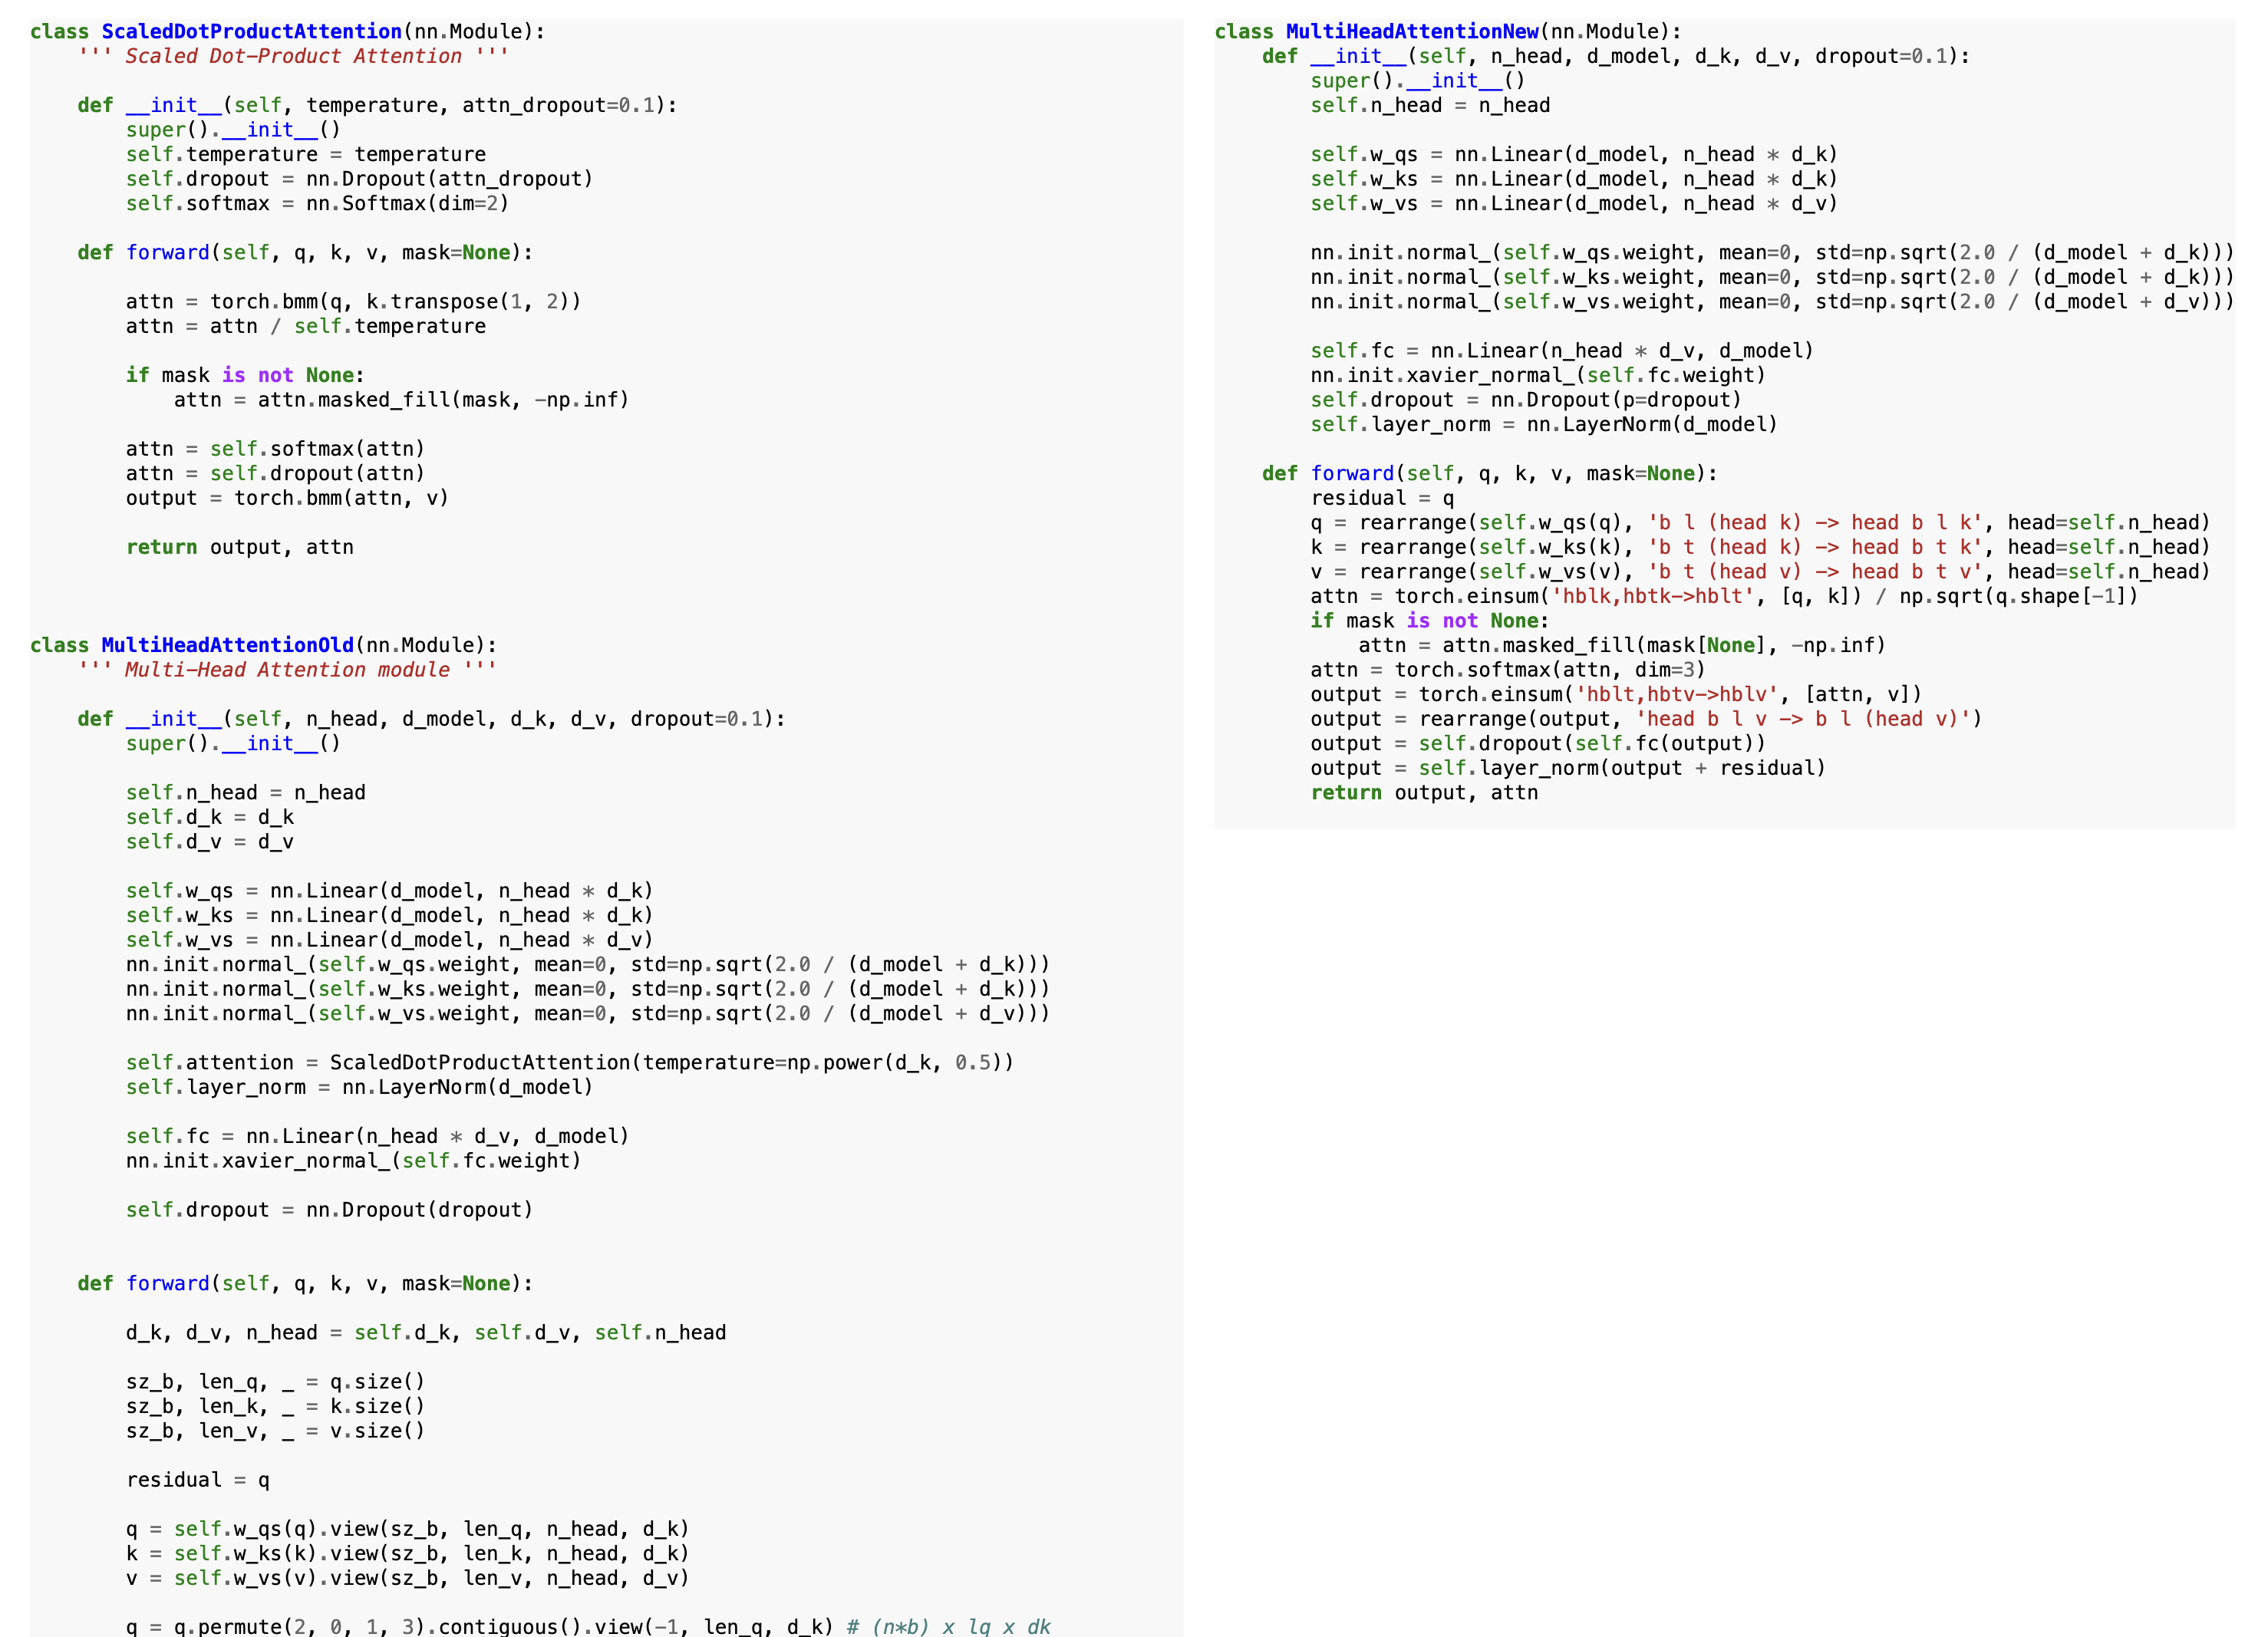
\includegraphics[width=\linewidth]{comparison}
			\end{figure}
		\end{column}
	\end{columns}
	\tiny{Credit: \url{https://einops.rocks/pytorch-examples.html}}
\end{frame}

\begin{frame}[fragile]{Einsum Implementation}
\begin{columns}
\column{0.48\textwidth}
\textbf{Matrix multiply:}

$C=$ \ein{$pq,qr \to pr; A, B$}
	
\begin{itemize}
	\item $C$ has dimensions $|p| \times |r|$
	\item $C_{pr} = \sum_q A_{pq}B_{qr}$
\begin{lstlisting}[language=python]
for p in range(P):
  for r in range(R):
    for q in range(Q):
      C[p,r] += A[p,q]*B[q,r]
\end{lstlisting}		
\end{itemize}
	
\pause
\column{0.55\textwidth}
\textbf{Batched matrix multiply + reduce:}

$C=$ \ein{$bpq,bqr \to br; A, B$}
\begin{itemize}
	\item $C$ has dimensions $|b| \times |r|$
	\item $C_{br} = \sum_{pq} A_{bpq}B_{bqr} = \sum_q B_{bqr} \sum_{p} A_{bpq}$
\begin{lstlisting}[language=C]
for b in range(B):
  for r in range(R):
    for p in range(P):
      for q in range(Q):
        C[b,r] += A[b,p,q]*B[b,q,r]
\end{lstlisting}
\end{itemize}
\end{columns}
\end{frame}

\begin{frame}[fragile]{Multi-Tensor Einsum Implementation}

\begin{columns}
\column{0.75\textwidth}
$D =$ \ein{$pq,qr,rs \to ps; A, B, C$}
\begin{itemize}
	\item $D_{ps} = \sum_{qr} A_{pq}B_{qr}C_{rs}$
	\begin{lstlisting}[language=C]
for p in range(P):
  for s in range(S):
    for q in range(Q):
      for r in range(R):
        D[p,s] += A[p,q]*B[q,r]*C[r,s]
\end{lstlisting}
\end{itemize}
\pause
The naive approach is inefficient!
This is $O(|p| \cdot |q| \cdot |r| \cdot |s|) \approx O(n^4)$.
\end{columns}
\end{frame}

\begin{frame}[fragile]{Multi-Tensor Einsum Implementation}

\begin{columns}
\column{0.75\textwidth}
\ein{$pq,qr,rs \to ps; A, B, C$} $=$ \ein{$pr, rs \to ps; AB, C$}, where $AB =$ \ein{$pq,qr \to pr; A, B$}.
\begin{itemize}
	\item $D_{ps} = \sum_{r} (AB)_{pr}C_{rs}$
	\begin{lstlisting}[language=C]
for p in range(P):
  for r in range(R):
    for q in range(Q):
      AB[p,r] += A[p,q]*B[q,r]
 
for p in range(P):
  for s in range(S):
    for r in range(R):
      D[p,s] += AB[p,r]*C[r,s]
\end{lstlisting}
\end{itemize}
\pause
This is $O(|p| \cdot |r| \cdot |q| + |p| \cdot |s| \cdot |r|) \approx O(n^3)$.
\end{columns}
\end{frame}

\begin{frame}{Contraction Paths}

\begin{columns}
\column{0.4\textwidth}
	Key idea: implement arbitrary einsum expressions by reducing them to binary einsums.
	
	\medskip
	New problem: there are many possible reductions; some are more efficient; finding optimal reduction is \textsf{NP}-hard.
	\begin{itemize}
		\item Cost models: max size of intermediate tensor; number of FLOPs.
		\item Despite \textsf{NP}-hardness, good heuristics exist.
	\end{itemize}
	

\column{.48\textwidth}
\ein{$pq,qr,rs,st \to pt; A,B,C,D$}

\medskip
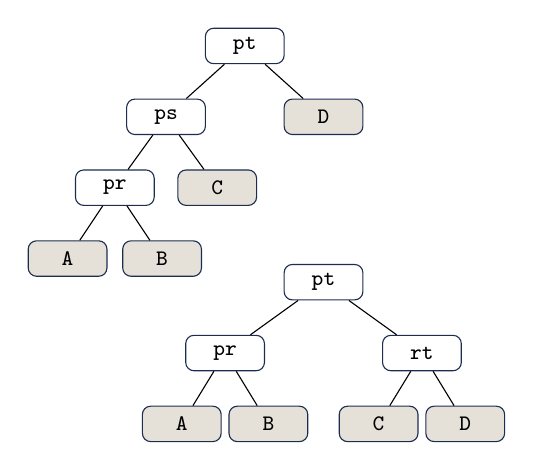
\begin{tikzpicture}[level distance=0.9cm,
    level 1/.style={sibling distance=2cm},
    level 2/.style={sibling distance=1.3cm},
    level 3/.style={sibling distance=1.2cm}]
  \node[tnode] {pt}
    child { node[tnode] {ps}
      child { node[tnode] {pr}
        child { node[tleaf] {A} }
        child { node[tleaf] {B} }
      }
      child { node[tleaf] {C} }
    }
    child { node[tleaf] {D} };
  %
  \begin{scope}[yshift=-3cm,
  xshift=1cm,
      level 1/.style={sibling distance=2.5cm},
      level 2/.style={sibling distance=1.1cm}]
    \node[tnode] {pt}
      child { node[tnode] {pr}
        child { node[tleaf] {A} }
        child { node[tleaf] {B} }
      }
      child { node[tnode] {rt}
        child { node[tleaf] {C} }
        child { node[tleaf] {D} }
      };
  \end{scope}
\end{tikzpicture}

\medskip
\hspace{5em} \small \textcolor{Crimson}{Contraction trees}
\vspace{-2em}
\end{columns}	
\end{frame}


\section{Tensor Processing Primitives}

\begin{frame}{Implementing Binary Einops}
	Once we've decided on a contraction path, we must implement the binary einops.
	
	Typically, this means executing matrix multiplies.
	
	And typically, \emph{that} means calling an optimized GEMM (GEneral Matrix Multiply) kernel from BLAS.\footnote{Basic Linear Algebra Subprograms, a library of optimized LA primitives written in Fortran.}
	\begin{itemize}
		\item The paper also uses packed GEMM (batched MM) and transpose.
		\item GEMM, packed GEMM, and transpose form the paper's \textbf{Tensor Processing Primitives}, into which einsum computations decompose. 
	\end{itemize}
	
\end{frame}

\begin{frame}{GEMM and Memory Layout}

GEMM assumes a specific data layout.

Each problem dimension is classified into one of the basic GEMM types: M, N, K, C, R.
\begin{itemize}
	\item [$\circ$] M/N: free dimensions preserved in output (present in single input and in output)
	\item [$\circ$] C: batch dimensions (in several inputs and in output)
	\item [$\circ$] K: reduced dimensions (in several inputs but not output; requires multiplication)
	\item [$\circ$] R: reduced dimensions (in single input and not output; only requires sum)
\end{itemize}
\end{frame}

\begin{frame}[fragile]{GEMM and Memory Layout}
	A GEMM call has the form \code{C[M][N] += A[M][K]*B[K][N]}.%\footnote{Note: the paper uses \code{C[N][M] += A[K][N]*B[M][K]}, because BLAS is written in Fortran, which is column-major. But I find the row-major formulation more intuitive.}
	
	A packed GEMM call has the form \code{C[C][M][N] += A[C][M][K]*B[C][K][N]}.
	
	BLAS\footnote{Basic Linear Algebra Subprograms, which implements GEMM.} requires the \code{N} and \code{K} dimensions to be contiguous in memory (i.e. to have stride 1).
	\begin{itemize}
		\item This enables SIMD vectorization and plays nicely with cache behavior and prefetching.
	\end{itemize}
	
	Thus, BLAS constrains the einsum dimensions to the format 
	
	\centering\code{(C)MK, (C)KN $\to$ (C)MN}.\footnote{Note: The paper uses \code{KMC, NKC $\to$ NMC} because BLAS is written in Fortran, which follows a column-major data layout. I've translated the requirement to a more C-friendly layout.}
	
%	Consider \ein{$pq,rq \to pr; A, B$}: the \code{K}-type dimension is $q$, which has stride 1 for $B$.
%	But BLAS requires the \code{N}-type dimension to have stride 1 for $B$.
\end{frame}

\begin{frame}{GEMM and Memory Layout}
BLAS requires \code{CMK, CKN $\to$ CMN}.
\bigskip
	\begin{columns}
	\column{0.4\textwidth}	
	\ein{$bij,bjk \to bik; A, B$}
	
	\begin{tabular}{ll}
	 	\toprule
		\textbf{Dimension} & \textbf{GEMM Type}\\
		\midrule
		$b$ & C \\
		$i$ & M \\
		$j$ & K \\
		$k$ & N \\
		\bottomrule
	\end{tabular}
	
	\medskip
	Order: \code{CMK, CKN $\to$ CMN}.
	
	\column{0.4\textwidth}
	\ein{$ab,ac \to cb; A, B$}
	
	\begin{tabular}{ll}
	 	\toprule
		\textbf{Dimension} & \textbf{GEMM Type}\\
		\midrule
		$a$ & K \\
		$b$ & M \\
		$c$ & N \\
		\bottomrule
	\end{tabular}	
	
	\medskip
	Order: \code{KM, KN $\to$ NM}.
	\end{columns}

\pause	
\medskip
The second example can be brought into GEMM-friendly layout by transposing $A$ and the output: \ein{$ba, ac \to bc; A^\top, B$}.
But this involves a potentially costly transpose on $A$.
	
\end{frame}

\begin{frame}
	
\end{frame}

\section{Einsum Trees}

\begin{frame}{General Solution}
	To solve the problem, the paper
	\begin{enumerate}[i)]
		\item enriches the representation of the contraction path into an \emph{einsum tree}, and
		\item systematically transforms the tree to make each binary einop GEMM-friendly.
	\end{enumerate}
\end{frame}

\begin{frame}{Einsum Trees}
The enriched representation is the \textbf{einsum tree}.
\begin{itemize}
 	\item Functions as an Intermediate Representation (IR), facilitating the analysis and optimization of the original einsum expression.
	\item Build upon \emph{contraction trees}, which simply record data dependencies among binary einsums.
	\item Einsum trees augment contraction trees with information about child node ordering and about dimension order within a node.
\end{itemize}
\end{frame}

\begin{frame}{Transformations}
	Three transformations:
	\begin{enumerate}
		\item Swap children of a node
		\item Reorder indices of a node
		\item Insert a permutation node
	\end{enumerate}
	Any einsum tree can be transformed into a GEMM-compatible one by applying these transformations.
\end{frame}

\begin{frame}{Algorithm}
	\textbf{Step 1:} assign a GEMM type to each problem dimension

	\textbf{Step 2:} transform einsum tree to make it GEMM-friendly:
	\begin{itemize}
		\item If $I_1$ has rightmost $N$ dimension and $I_2$ has rightmost $M$ dimension, swap them.
		\item Reorder indices within nodes to satisfy GEMM requirements (\code{CMK} for left children, \code{CKN} for right children).
		\item Insert permutation nodes below reordered nodes.
	\end{itemize}
\end{frame}


\begin{frame}{Example}
	\ein{$ij,jk,im \to km$}
	\bigskip
	
	\begin{columns}
	\column{0.25\textwidth}	
	Contraction tree:
	
	\vspace{1em}
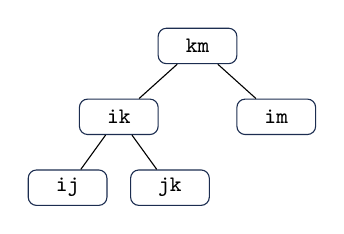
\begin{tikzpicture}[level distance=0.9cm,
    level 1/.style={sibling distance=2cm},
    level 2/.style={sibling distance=1.3cm},
    level 3/.style={sibling distance=1.2cm}]
    \begin{scope}[yshift=-2cm]
    	 \node[tnode] {km}
    child { node[tnode] {ik}
      child { node[tnode] {ij}
      }
      child { node[tnode] {jk} }
    }
    child { node[tnode] {im} };

    \end{scope}
 
\end{tikzpicture}

\column{0.25\textwidth}

Reorder indices:

	\vspace{1em}
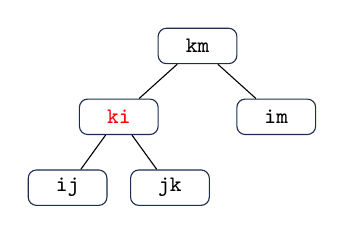
\begin{tikzpicture}[level distance=0.9cm,
    level 1/.style={sibling distance=2cm},
    level 2/.style={sibling distance=1.3cm},
    level 3/.style={sibling distance=1.2cm}]
    \begin{scope}
      \node[tnode] {km}
    child { node[tnode] {{ \color{red} ki }}
      child { node[tnode] {ij}
      }
      child { node[tnode] {jk} }
    }
    child { node[tnode] {im} };
    \end{scope}
\end{tikzpicture}

\column{0.25\textwidth}

Swap children:

	\vspace{1em}
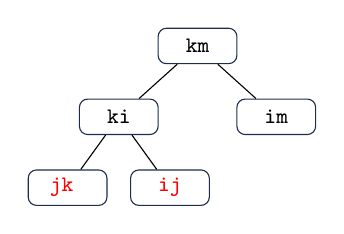
\begin{tikzpicture}[level distance=0.9cm,
    level 1/.style={sibling distance=2cm},
    level 2/.style={sibling distance=1.3cm},
    level 3/.style={sibling distance=1.2cm}]
    \begin{scope}
      \node[tnode] {km}
    child { node[tnode] {{ki}}
      child { node[tnode] {{\color{red} jk }}
      }
      child { node[tnode] {{ \color{red} ij }} }
    }
    child { node[tnode] {im} };
    \end{scope}
\end{tikzpicture}
\column{0.25\textwidth}

\vspace{2.5em}
Insert permutation:

	\vspace{1em}
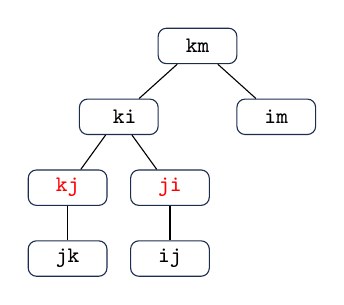
\begin{tikzpicture}[level distance=0.9cm,
    level 1/.style={sibling distance=2cm},
    level 2/.style={sibling distance=1.3cm},
    level 3/.style={sibling distance=1.2cm}]
    \begin{scope}
      \node[tnode] {km}
    child { node[tnode] {{ ki}}
      child { node[tnode] {{ \color{red}kj }} child { node[tnode] {jk} }
      }
      child { node[tnode] {{ \color{red} ji }} child { node[tnode] {ij} } }
    }
    child { node[tnode] {im} };
    \end{scope}
\end{tikzpicture}


	\end{columns}

\end{frame}

\section{Results}

\begin{frame}{Evaluations}
	Comparison to: TVM-Ansor, ATen (pytorch), OE-Torch on TCCG benchmark.
\begin{center}
\begin{figure}
	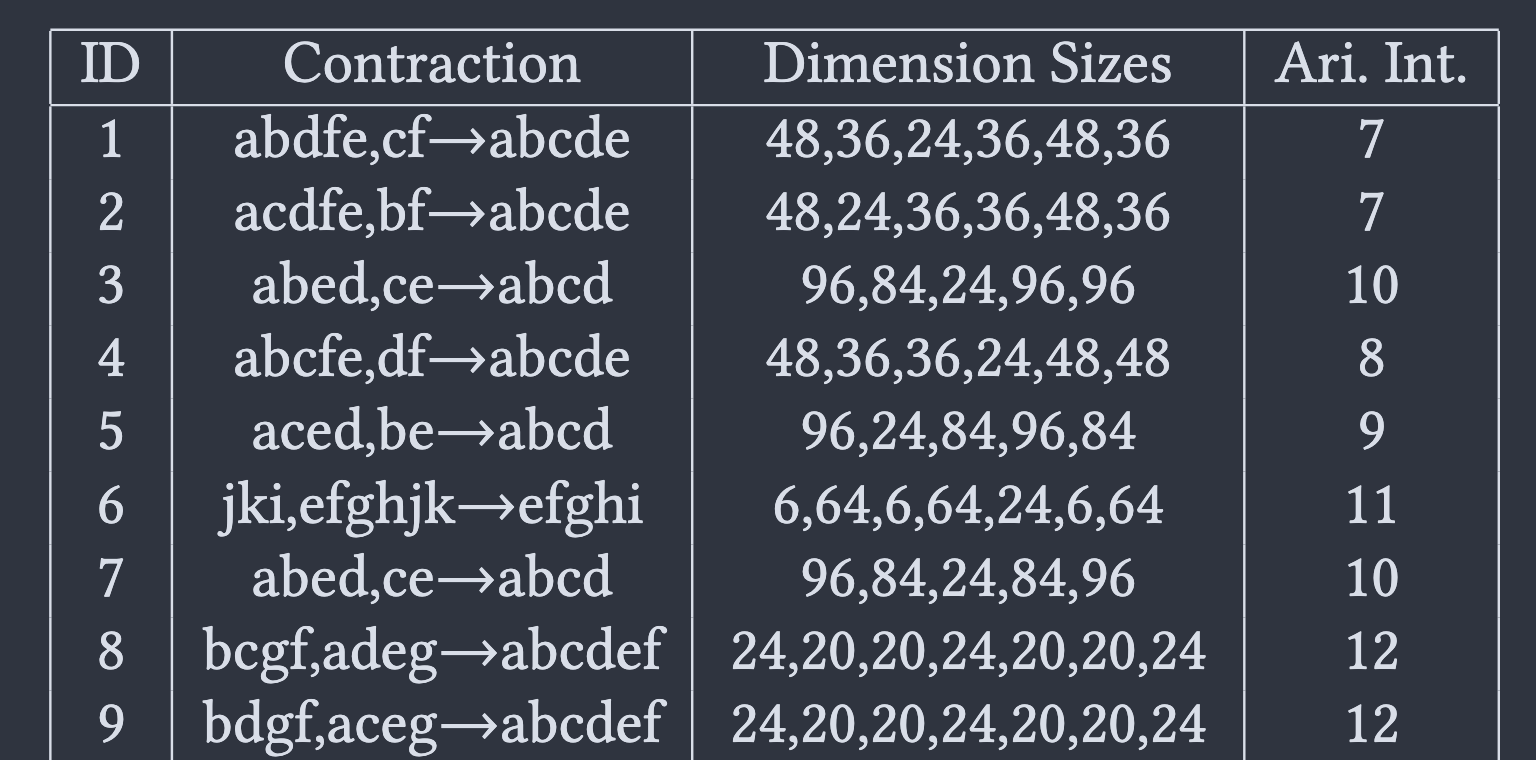
\includegraphics[width=0.49\textwidth]{binary_contractions.png}	
	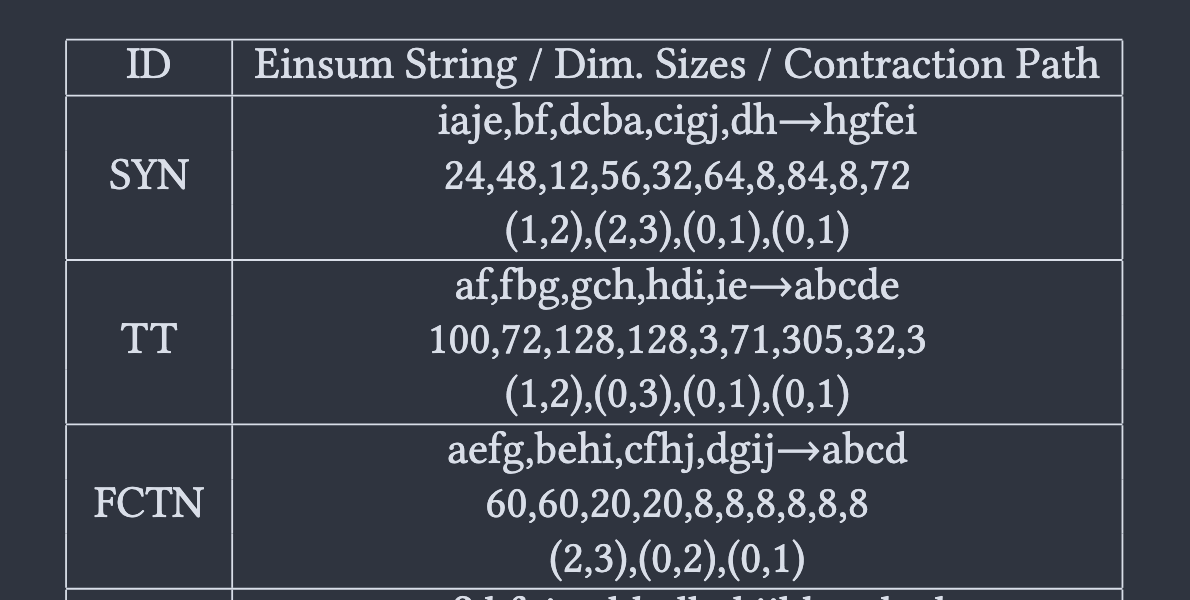
\includegraphics[width=0.49\textwidth]{benchmark_trees.png}
\end{figure}
\end{center}
\hspace{4em} Binary Contractions \hspace{12em} Contraction Trees

\end{frame}

\begin{frame}{FLOPs}
	\begin{center}
	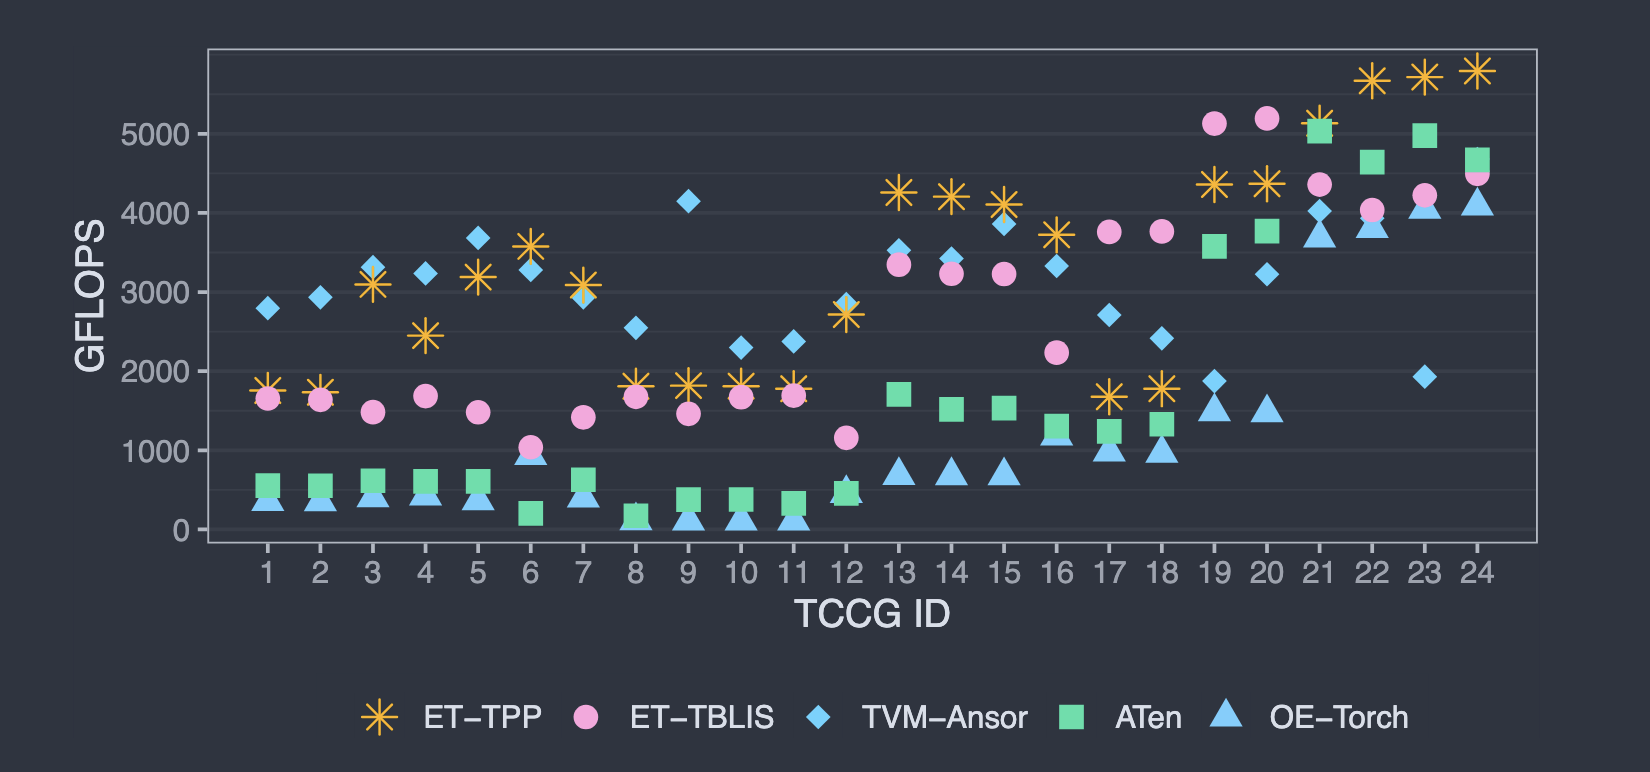
\includegraphics[width=0.8\textwidth]{perf_plot.png}
	\end{center}
\end{frame}

\begin{frame}{Compilation Time}
\begin{center}
	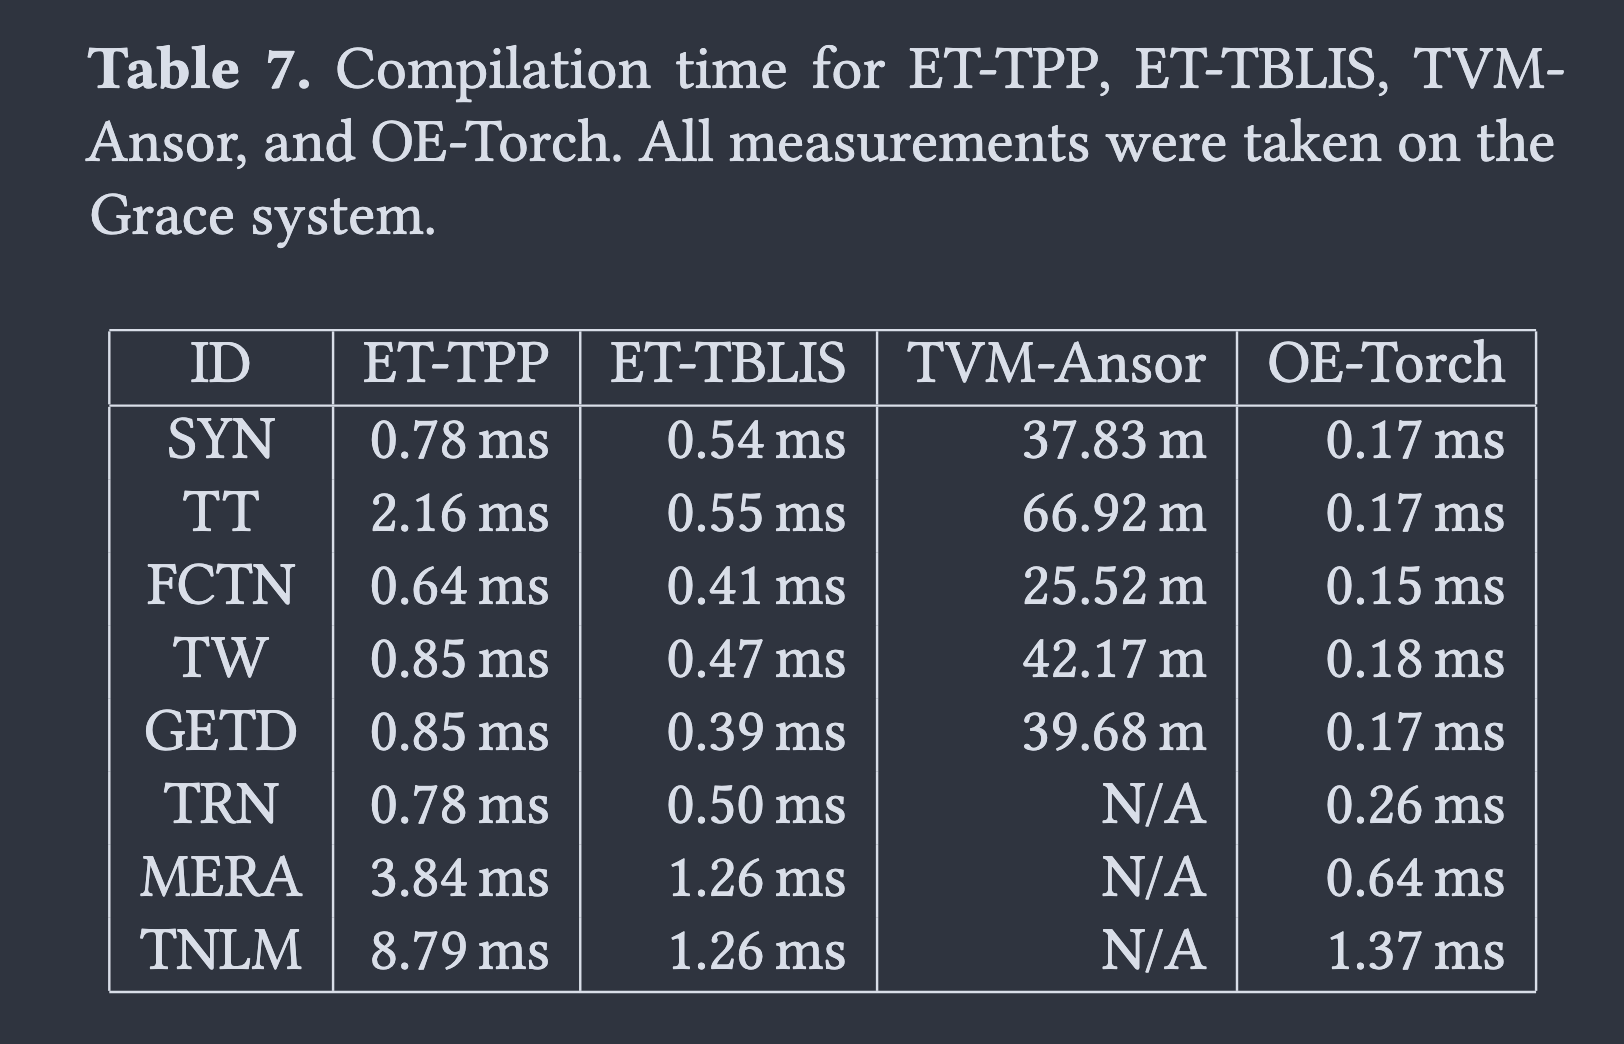
\includegraphics[width=0.7\textwidth]{compile_time}
\end{center}
	
\end{frame}

\begin{frame}{Summary of Results}
	\begin{itemize}
		\item Comparable or superior performance on most benchmark problems.
		\item Vastly better compilation time than TVM-Ansor.
	\end{itemize}
\end{frame}

\section{Limitations and Questions}

\begin{frame}{Limitations and Questions}
	\begin{enumerate}
		\item The optimization algorithm is presented without any analysis. Is it optimal? Does it fail on certain cases?
		\item Contraction paths are given. But perhaps contraction path and layout optimization need to be jointly optimized?
		\item Some liberties taken with the benchmark.
		\item CPU-only.
	\end{enumerate}
\end{frame}


















\end{document}